\chapter{bf16数据同步方法}
本章主要介绍bf16数据同步方法的实现原理。并将详细介绍整个框架工作流程和性能优化的相关方法。通过分析不同应用的理论效率和实际效率结果,评估系统的性能。
\section{引言}
随着人工智能的快速发展,为提升训练效率,满足生产需求,业界已针对分布式深度学习系统进行了深入的研究。本章希望通过压缩模型梯度数据的方式来减少分布式同步数据过程中的数据传输量,以此减小同步时间开销,提高分布式训练效率。本章将介绍如何在现有高效的分布式通信框架horovod上集成现有主流的深度学习框架,并进一步实现bf16的数据通信方法;并介绍通过优化实现得到的性能提升,最后通过理论分析和实验结果比较,说明bf16数据同步方式的有效性和实用性。
\section{框架设计}
\subsection{MXNet与Horovod的整合}
horovod上uber针对tensorflow在分布式深度学习训练中的不足,基于百度提出的ring-allreduce[引用]构建。有3个主要特征[引用horovod]:\\
1. horovod与深度学习框架相互独立,用户以python包的形式调用horovod的API。使其发展独立于任何深度学习框架,目前horovod已经支持tensorflow和pytorch。这样tensorflow和pytorch用户可以在任意版本的深度学习框架中使用horovod,不需要担心兼容问题。目前MXNet团队已经将MXNet整合进了horovod,正在等待horovod团队整合。\\
2. 用NCCL取代了百度ring-allreduce实现。NCCL是NVIDIA的集体通信库,提供高度优化的ring-allreduce实现。通过NCCL的ring-allreduce实现,使得horovod的性能有巨大提升。\\
3. 提出tensor fusion方法,通过将多个小的tensor整合成数据量稍大的tensor,进而对这个大的fusion做allreduce。提高了数据的通信效率。\\
\begin{figure}[htp]
\centering
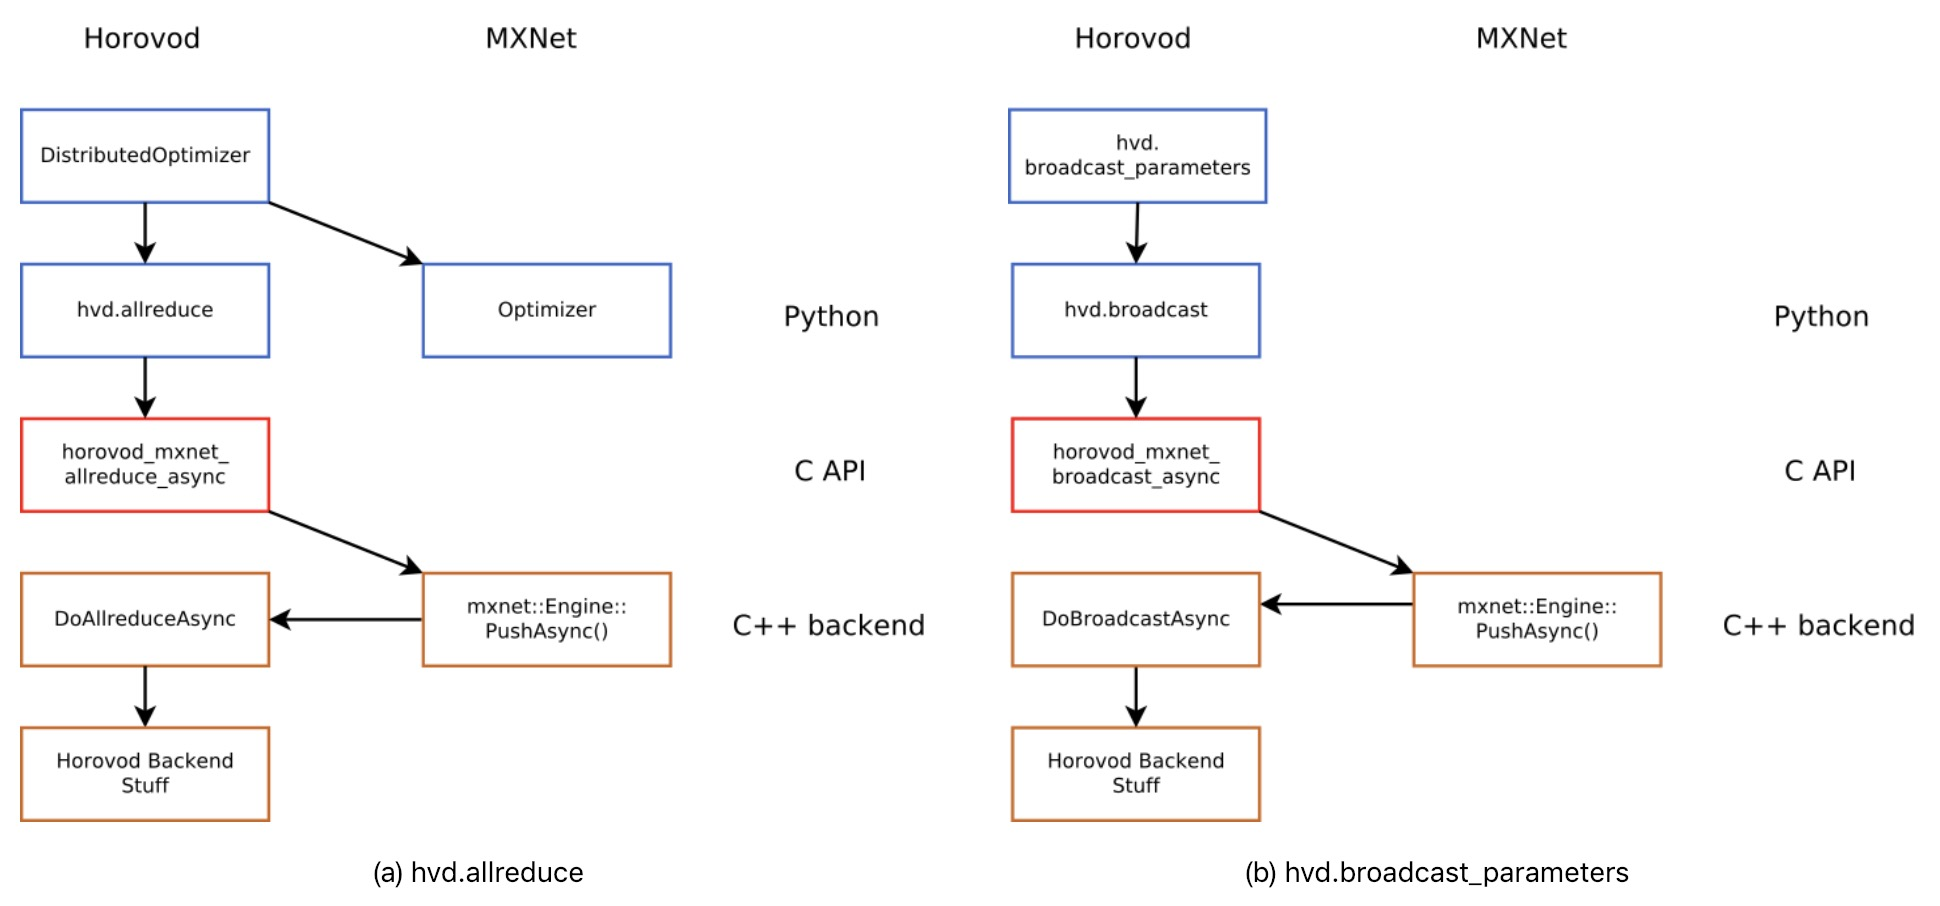
\includegraphics[width=10cm]{horovod_mxnet_integration}
\caption{MXNet与horovod整合示意图}
\end{figure}
horovod中主要涉及两个操作:allreduce和broadcast。其与MXNet的整合示意图如图3.1所示。由图可知,horovod通过继承MXNet的优化器optimizer实现与mxnet的整合,即更新模型时使用horovod的DistributedOptimizer更新。对于MXNet而言,分布式程序只是一个使用DistributedOptimizer优化器更新模型的单机程序。在horovod中,因为其在真正更新之前,会对参数做allreduce来同步全局参数。这种整合方式使得mxnet与horovod可以各自独立发展,二不会产生版本的相互依赖。为保证各个节点中初始化的模型一致, 其提供了一个 broadcast parameters的API用于同步模型初始化的值。\\
horovod通过对外提供tensor接口,使得更深度学习框架能整合进horovod中。接口如下所示:
\begin{lstlisting}[language=C, numbers=none]
Tensor {
  dtype();  //  return the data type of tensor;
  shape();  //  return the shape of tensor;
  data();   //  return the data pointer of tensor;
  size();   //  return the total bytes of data;
}
\end{lstlisting}
由上伪代码可知,将深度学习框架整合进horovod只需通过继承tensor这个基类并实现对应的方法即可。而horovod只需通过调用tensor中的对应方法即可。故为将mxnet整合入horovod,其设计如下:
\begin{lstlisting}[language=C, numbers=none]
MXTensor : Tensor{
public:
  MXTensor(NDArray* tensor);
  // override the 4 APIs
  dtype();
  shape();
  data();
  size();
protected:
  NDArray* tensor_;  // the pointer address to the data from MXNet
}
\end{lstlisting}
\subsection{在horovod上实现bf16}
由第二章介绍可知,bf16计算需要硬件支持,目前只有google的TPU支持该计算,对应地tensorflow对其支持。但其他主流框架如pytorch,mxnet没有完全支持bf16的数据格式,故目前bf16只能作为一种数据压缩方式用于分布式深度学习训练中。基于mxnet,在horovod上实现bf16数据通信的方法主要包含三部分:1.继承horovod提供的Tensor,设计bf16 Tensor供horovod调用;2.实现一个自定义的bf16求和函数,供MPI做allreduce时对bf16数据求和时使用;3.在对bf16做完allreduce后,将bf16数据转换成fp32数据。\\
针对以上三部分内容,具体设计如下所示:
\begin{lstlisting}[language=C, numbers=none]
// 1. bf16 tensor defination
MXBF16Tensor: MXTensor {
public:
  MXBF16Tensor(NDArray* tensor):MXTensor(tensor){
  // according the count of tensor elements allocate memory to store bf16 data;
  // convert source data of tensor to bf16 data format
}
  source_data();   // return the source pointer of NDArray;
  // override the 3 APIs as below:
  dtype();  // return bf16 flag;
  data();    // return data pointer of bf16;
  size();     // return the total bytes of bf16 data;
  private:
  unsigned short* bf16dptr_;
}

// 2. implement bf16 sum according MPI_op define
void bf16_sum(void* invec, void* inoutvec, int* len, MPI_Datatype* datatype) {
  for(int i = 0; i < *len; i++) {
    float tmp_in = convert_bf16_to_fp32(invec[i]);
    float tmp_out = convert_bf16_to_fp32(inoutvec[i]);
    tmp_out += tmp_in;
    inoutvec[i] = convert_fp32_to_bf16(tmp_out);
  }
}

// 3. convert bf16 data to fp32 data on callback function.
void callback() {
        // convert bf16_tensor to fp32, assign to output
        mxnet.tensor.dptr = BF16ToFloat(bf16_pointer, len);
        handle_manager.MarkDone(handle);
        handle_manager.ExecuteCallback(handle);
      }
\end{lstlisting}
\section{性能优化}
为减小fp32数据与bf16数据的转换开销和bf16 sum中计算效率,我们通过使用instrinsic指令直接操作数据完成数据转换和计算。针对不同情况,进行了最优实现,使用AVX512指令进行转换的实现如下所示:
\begin{lstlisting}[language=C, numbers=none]
inline void convert_f32_to_b16(const void* src, void* dst)
{
  __m512i y = _mm512_bsrli_epi128(_mm512_loadu_si512(src), 2);
  _mm256_storeu_si256((__m256i*)(dst), _mm512_cvtepi32_epi16(y));
}

inline void convert_f32_to_b16(__m512i* src, __m256i* dst)
{
  __m512i y = _mm512_bsrli_epi128(*src, 2);
  *dst = _mm512_cvtepi32_epi16(y);
}

inline void convert_b16_to_f32(const void* src, void* dst)
{
  __m512i y = _mm512_cvtepu16_epi32(_mm256_loadu_si256((__m256i const*)src));
  _mm512_storeu_si512(dst, _mm512_bslli_epi128(y, 2));
}
\end{lstlisting}
\section{理论分析}
1. resnet50理论计算量与计算时间

\begin{table}[htbp]
  \centering
  \caption{网络模型分析}
  \label{tab:tabexamp1}
  \begin{minipage}[t]{0.8\textwidth} 
    \begin{tabularx}{\linewidth}{|l|X|X|X|X|X|X|X|X|X|}
      \hline
      \multirow{2}*{\backslashbox{模型}{时间}}& \multicolumn{3}{c|}{Forward}& \multicolumn{3}{c|}{Backward}& \multicolumn{3}{c|}{Update}\\
      \cline{2-10}
      &计算量 &理论时间 &实际时间 &计算量 &理论时间 &实际时间 &计算量 &理论时间 &实际时间\\ 
      \hline
      resnet50& 20.4& 27.4& 90& 20.4& 27.4& 90& 20.4& 90& 20.4\\
      SSD&      20.4& 27.4& 90& 30.6& 38.6& 34.6& 31.6& 90& 20.4\\ 
      GNMT&     20.4& 27.4& 90& 30.6& 38.6& 34.6& 31.6& 90& 20.4\\ 
      \hline
    \end{tabularx}\\[2pt]
    \footnotesize
    *:东部\\
    **:西部
  \end{minipage}
\end{table}


comm time \\
comp time
\section{结果分析}




精度,性能(classification, detection, nlp)